% autobench --single_host --host1 with_naxsi.test.nl --uri1 /index.php --low_rate 1 --high_rate 130  --rate_step 5 --const_test_time 30  --file results.csv

\documentclass[Measurements]{subfiles}
\begin{document}
\section{Measurements}
\label{sec:Measurements}
Basically, there are two main different scenarios for measuring the performance. The first one is by measuring the performance of Nginx when Naxsi is disabled. The second one is by measure the performance when Naxsi is enabled. First, a baseline performance measurement is performed. The baseline is used as a reference for the other performance measurements. Second, the performance of Naxsi is measurement by changing the number of rules.

\subsection{Baseline performance measurement}
In order to measure the performance of Naxsi, it is important to know the bottleneck of the back-end server doing all the processing at the application layer. Figure \ref{fig:Baseline measurement 1} shows that $\approx 21\%$ of the 10,000 requests produce a \verb+HTTP 5xx+ response when using 250 concurrent connections. Details can be found in appendix \ref{sec:baseline_measurement_1}

\begin{table}[!h]
\caption{Baseline measurement 1}
\begin{tabular}{|p{2cm}|p{1,5cm}|p{1,5cm}|p{1,5cm}|p{1,5cm}|p{1,5cm}|}
\hline
 & \textbf{1xx} & \textbf{2xx} & \textbf{3xx} & \textbf{4xx} & \textbf{5xx} \\ \hline
\textbf{Connections} & 0 & 0 & 8542 & 0 & 1458 \\ \hline
\end{tabular}
\label{fig:Baseline measurement 1}
\end{table}

By using a half-interval search method, the optimal number of concurrent connections, which gave the highest rate of 190 request per second. As can be seen in figure \ref{fig:Baseline measurement 2}, the total number of \verb+HTTP 3xx+ responses is 10,000. Details can be found in appendix \ref{sec:baseline_measurement_2}

\begin{table}[h]
\caption{Baseline measurement 2}
\begin{tabular}{|p{2cm}|p{1,5cm}|p{1,5cm}|p{1,5cm}|p{1,5cm}|p{1,5cm}|}
\hline
 & \textbf{1xx} & \textbf{2xx} & \textbf{3xx} & \textbf{4xx} & \textbf{5xx} \\ \hline
\textbf{Connections} & 0 & 0 & 10000 & 0 & 0 \\ \hline
\end{tabular}
\label{fig:Baseline measurement 2}
\end{table}

Based on the values derived from the measurement above, the performance is measured by stepping through the concurrent connections from 1 to 190. The response time is calculated by taking the average of each measurement of  each step. Each step has a measurement duration of 60 seconds. 

% autobench --single_host --host1 wp_without_naxsi.test.nl --uri1 /index.php --low_rate 1 --high_rate 230 --rate_step 1 --num_call 1 --const_test_time 60 --file results.csv
\begin{figure}[H]
\caption{Autobench baseline performance measurement}
\centering
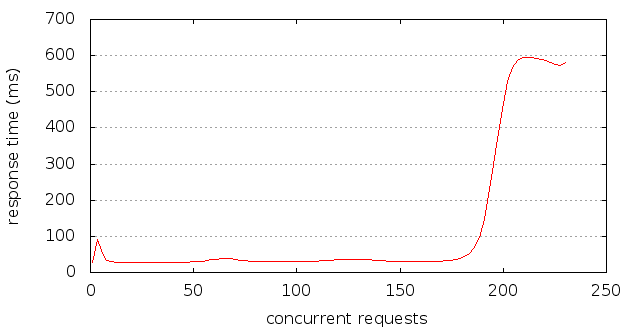
\includegraphics[scale=0.55] {images/results/baseline/output.png}
\label{fig:Baseline performance measurement}
\end{figure}

When staying under 190 concurrent connections, the response time is \mbox{$\approx 30 ms$}. Figure \ref{fig:Baseline Nginx CPU usage} shows a steady increase of the number of jiffies when the numbers of concurrent connections increase. The number of jiffies only increase when the number of concurrent connections is still below 190. As soon as the concurrency raises above 190, the Nginx server starts returning \verb+HTTP 5xx+ error codes, because the back-end is not able to handle all requests. The memory foot print of Nginx is little, as can be seen in figure \ref{fig:Baseline Nginx memory usage}. The number of request have only a minimal impact on the memory usage. The number Bytes written on disk is also very minimal, as can be seen in figure \ref{fig:Baseline Nginx disk traffic}. Around 21.30 hours the disk IO drops slighty, which is the time the measurement ended. Figure \ref{fig:Baseline Nginx interface traffic} also shows that there is little network traffic. The number of received bits increments linearly as expected, because of incremental number of request received from server04.   

\begin{figure}[H]
\centering
\caption{Baseline Nginx CPU usage}
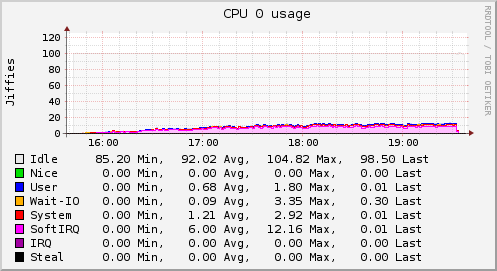
\includegraphics[scale=0.7]{images/results/baseline/cpu.png}
\label{fig:Baseline Nginx CPU usage}
\end{figure}

\begin{figure}[H]
\centering
\caption{Baseline Nginx memory usage}
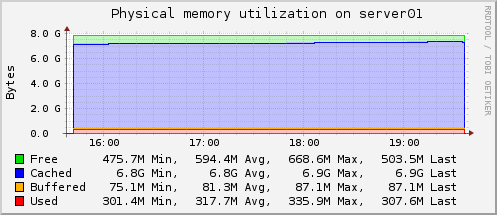
\includegraphics[scale=0.7]{images/results/baseline/memory.png}
\label{fig:Baseline Nginx memory usage}
\end{figure}

\begin{figure}[H]
\centering
\caption{Baseline Nginx disk traffic}
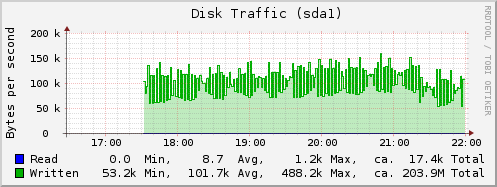
\includegraphics[scale=0.7]{images/results/baseline/disk.png}
\label{fig:Baseline Nginx disk traffic}
\end{figure}

\begin{figure}[H]
\centering
\caption{Baseline Nginx interface traffic}
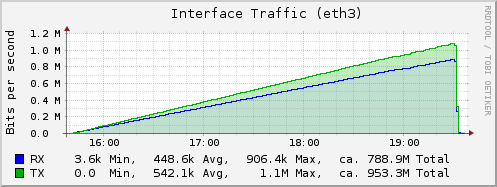
\includegraphics[scale=0.7]{images/results/baseline/interface.png}
\label{fig:Baseline Nginx interface traffic}
\end{figure}

\subsection{Naxsi performance measurement}

After enabling Naxsi in \verb+/etc/nginx/nginx.conf+ and after reloading Nginx, it is possible to do the performance measurement of Nginx combined with Naxsi. Details about how to enable Naxsi can be found in appendix \ref{sec:server01_configuration}. All Naxsi performance measurements include the Naxsi core rules. Because Naxsi uses a white listing mechanism, the performance test of Naxsi is measured by incrementing the number of rules on the site level configuration. Each request should be passed through the white list and based on the final score, Naxsi either allows or denies the request. The denied request, in this setup, simply returns an \verb+HTTP 403+ error code. Both \verb+/var/log/nginx/access.log+ and \verb+/var/log/nginx/error.log+ can be monitored to see what Naxsi does with the request.

\subsubsection{Naxsi zero rules}
The initial performane measure with Naxsi includes only a simple subset of site rules. Details can be found in appendix \ref{sec:Naxsi measurement 1}.

\subsection{Naxsi performance measurement}
\end{document}

